
%%%%%%%%%%%%%%%%%%%%%%% file typeinst.tex %%%%%%%%%%%%%%%%%%%%%%%%%
%
% This is the LaTeX source for the instructions to authors using
% the LaTeX document class 'llncs.cls' for contributions to
% the Lecture Notes in Computer Sciences series.
% http://www.springer.com/lncs       Springer Heidelberg 2006/05/04
%
% It may be used as a template for your own input - copy it
% to a new file with a new name and use it as the basis
% for your article.
%
% NB: the document class 'llncs' has its own and detailed documentation, see
% ftp://ftp.springer.de/data/pubftp/pub/tex/latex/llncs/latex2e/llncsdoc.pdf
%
%%%%%%%%%%%%%%%%%%%%%%%%%%%%%%%%%%%%%%%%%%%%%%%%%%%%%%%%%%%%%%%%%%%


\documentclass[runningheads,a4paper]{llncs}

\usepackage{amssymb}
\setcounter{tocdepth}{3}
\usepackage{graphicx}
\usepackage{booktabs}
\usepackage{float}
\usepackage{url}
\urldef{\mailsa}\path|{rafael.possas, ying.zhou}@sydney.edu.au|    
\newcommand{\keywords}[1]{\par\addvspace\baselineskip
\noindent\keywordname\enspace\ignorespaces#1}

\begin{document}

\mainmatter  % start of an individual contribution

% first the title is needed
\title{Effectiveness of adversarial examples on class-imbalanced Convolutional Neural Networks}
\titlerunning{Imbalanced Learning and Adversarial Examples}
% a short form should be given in case it is too long for the running head

% the name(s) of the author(s) follow(s) next
%
% NB: Chinese authors should write their first names(s) in front of
% their surnames. This ensures that the names appear correctly in
% the running heads and the author index.
%
\author{Rafael Possas, Ying Zhou}
%
\authorrunning{Imbalanced Learning and Adversarial Examples}
% (feature abused for this document to repeat the title also on left hand pages)

% the affiliations are given next; don't give your e-mail address
% unless you accept that it will be published
\institute{University Of Sydney, Camperdown, NSW \\
\mailsa\\
\url{https://sydney.edu.au}}

%
% NB: a more complex sample for affiliations and the mapping to the
% corresponding authors can be found in the file "llncs.dem"
% (search for the string "\mainmatter" where a contribution starts).
% "llncs.dem" accompanies the document class "llncs.cls".
%

\toctitle{Lecture Notes in Computer Science}
\tocauthor{Authors' Instructions}
\maketitle


\begin{abstract}
A considerable amount of literature was published on the performance of Convolutional Neural Networks and the field has evolved considerably in the last years. However, as most machine learning methods, these networks suffer from the data imbalance problem - when the underlying training dataset is comprised of unequal number of samples for each label/class. Such difference naturally causes a phenomenon known as domain shift, which can be explained by the low generalisation capabilities of a model when presented with previously unseen data. Recent research have focused on a technique called Gradient Sign that forces domain shift on deep networks by creating adversarial examples. These are usually comprised of small directed changes on original data points that causes inputs to be misclassified by the predictive algorithm. Recent developments in such methods have heightened the need for better understanding of this phenomena. This study focuses on an experimental approach that sheds light on the link between the imbalanced learning problem and adversarial examples. Through a series of experiments we evaluated the gradient sign methods on imbalanced datasets linking their effectiveness with the underlying data distribution of image recognition models.
\keywords{convolutional neural networks, adversarial examples, gradient sign, imbalanced training}
\end{abstract}


\section{Introduction}

To date, little evidence has been found associating training data characteristics of a model with its robustness to adversarial examples. Experimental demonstrations of adversarial effects were carried out mainly by \cite{billovits}, \cite{goodfellow2014}, \cite{goodfellow2016}, \cite{papernot2016}. The motivation for Adversarial robustness comes largely from being able to shield image recognition systems from behaving unexpectedly. Previous published studies are limited to showing the general effectiveness of adversarial methods rather then understanding the deep relationship with the underlying training data distribution.

This work presents a practical approach for evaluation of gradient sign methods on datasets with skewed distributions. The main contributions of this work are as follows:
\begin{enumerate}
\item Understanding of the relationship between the gradients learned on an image recognition model and its vulnerability to gradient sign methods
\item Evaluation of the resilience of imbalanced CNNs to adversarial attacks using same model knowledge and transfer learning from different models.
\item Investigation of classes with similar distributions and their relationship to both adversarial attacks and imbalanced learning problem.
\end{enumerate}

Section 2 of this paper discusses the related work in both convolutional neural networks and gradient sign methods. Section 3 provides details of the training models, imbalanced datasets and gradient sign methods used in our experiments. Section 4 presents the results on the under-sampled, over-sampled and balanced cases using both same/different model gradient. Sections 5 and 6 are dedicated to drawing conclusions and providing directions to related future work.


\section{Related Work}

Recent work has shown that the generalisation capabilities of deep networks is rather sparse \cite{goodfellow2016}, \cite{papernot2016transf}. Thus, there is an opportunity for methods to exploit empty pockets of space and, hence, systematically create an adversary that produces an incorrect, high confidence prediction for an image without visible distortion. This can be done by adding just enough intentional noise to each pixel of the image so as to fool an algorithm into thinking that the image has an incorrect label \cite{goodfellow2014}, \cite{goodfellow2016}, \cite{papernot2016transf}, \cite{szegedy2013}.

The Gradient Sign method developed by Goodfellow et al. (2014) has been used as the foundation of many of the experiments in adversarial crafting on CNNs. The results have shown that the model can possibly have linear behavior in very high dimensional spaces.  Most inputs were miss-classified not only by Goodfellow et. al \cite{goodfellow2014}  experiments but many others \cite{billovits},\cite{goodfellow2016},\cite{papernot2016}.

Developing robustness to adversarial examples has already been approached as academic work \cite{billovits}, recent research has shown that one can use transfer learning to perform black-box attacks against Deep Neural Networks \cite{yosinski2014transferable} , \cite{papernot2016} .The combination of adversaries and transfer learning creates a threat vector for many state of the art methods. Attacks can, however, depend on some specific internal information of the target model \cite{papernot2016transf}. As most recent applied methods depend on the network gradient information, there is a straight dependence on the network confidence per class label and the robustness of the model to adversarial attacks.

Imbalanced learning is a well known cause for lower performance of several machine learning algorithms \cite{japkowicz2002class}, \cite{krawczyk2016learning}. Data distribution on real world is often skewed and rarely contains enough information to learn all the required features of the data domain. Adversaries are proven to explore class distributions vicinities, and the question whether imbalanced training sets affects their effectiveness is still unanswered.


\section{Initial Setup}

For the purposes of this work, we used a dataset that is not only visually rich but also enables analysis between different class labels. The 2014 ImageNet dataset \cite{deng2009imagenet} would be the natural choice, however, the amount of classes (1,000) would make it harder to perform comparisons. We use a dataset with similar characteristics, the CIFAR-10 \cite{krizhevsky_2009}. It contains 10 different class labels of 32x32 images, which enables us to easily train our algorithm from scratch and also to understand deeper relationships between labels.
\subsection{Network Architecture and parameters}

All the experiments were done using the VGG architecture \cite{simonyan2014very}. The two FC-4096 layers at the end were replaced by one single layer with 512 neurons and RELU activations. In addition, the total number of convolutions blocks and pooling were reduced to 3, with the first layer having 2 stacked convolution layers followed by a max pooling of stride 2x2 and the last two layers with 3 stacked convolutions also followed by a max pooling of stride 2x2. We have used RMSProp  \cite{bengiormsprop} as the optimisation technique with a learning rate of $10^{-4}$ and the decay $10^{-5}$. Figure~\ref{fig:conf_matrix_full} shows the results of our models on the CIFAR10 original dataset.

\begin{figure}
	\centering
	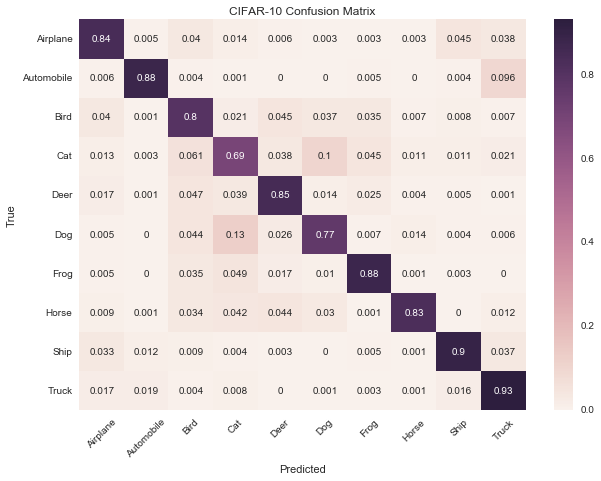
\includegraphics[height=6.0cm]{conf_matrix.png}
	\caption{Results of our adapted VGG architecture on CIFAR-10 dataset}
	\label{fig:conf_matrix_full}
\end{figure}

\subsection{Synthetic data imbalance}

As the CIFAR10 dataset is not naturally imbalanced, we have artificially created two variations on which we trained our networks.  While one dataset consisted on a direct under-sample of the target class to 1,000 samples, the other was changed using  an oversampling of the target class(or an under-sampling of all other classes). We kept the number of samples for the target class at 5,000 while all other classes were reduced to 1,000 samples. For each class of the two different datasets configurations, a network was then trained until convergence using the same hyper-parameters as the balanced case. Each model was evaluated against a test set of 10,000 equally distributed samples with the target class being perturbed by its own under/over-sampled model and the balanced model. Both imbalanced networks were separately tested for each class for both same model and different model adversaries. The same model test aims to understand the vulnerability of class imbalance on adversarial examples while the different model test main goal is to verify the robustness on transfer learning environments. In total we evaluated 50 different combinations: 20 for each different imbalanced dataset (same model gradient and balanced network gradient) and 10 for the balanced network using its own gradients on each class. Figure~\ref{fig:acc_graph} shows the accuracy for the models without any perturbation.
\begin{figure}
	\centering
	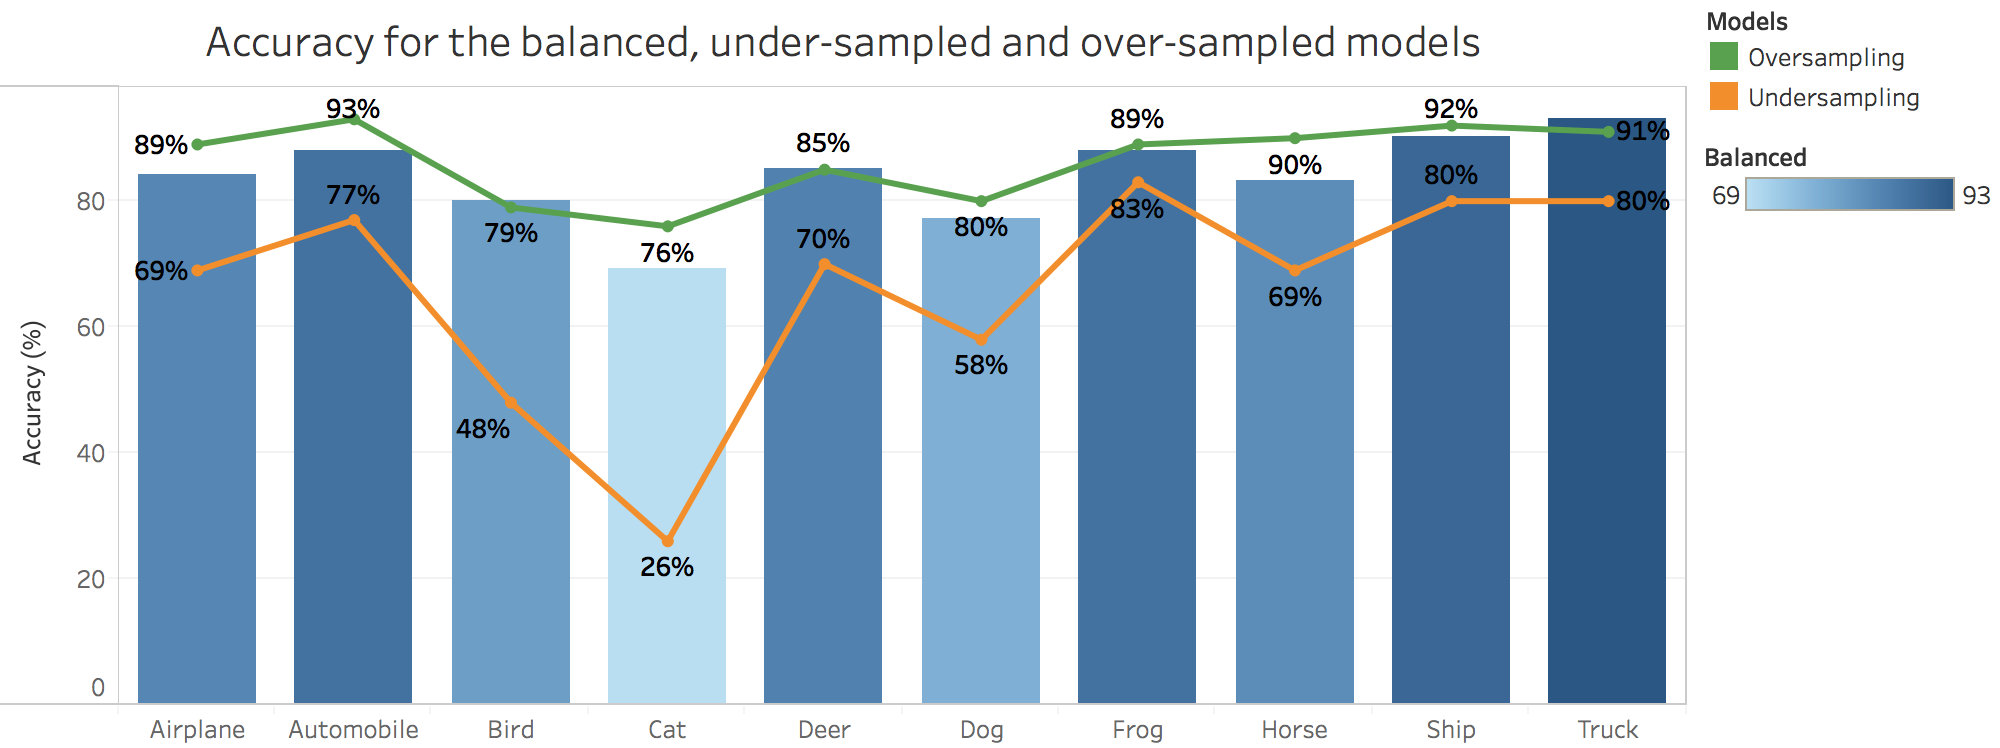
\includegraphics[height=5.5cm]{graph_non_pert.png}
	\caption{Target class accuracy on all models}
	\label{fig:acc_graph}
\end{figure}



\subsection{Gradient Sign methods}

The Gradient Sign is a method that uses internal gradient information so as to create directed perturbation to test data. Whether one adds or subtract noise according to equations 1 and 2, the resulting label will have different meanings. Suppose the current true label of the class is selected as a gradient candidate, adding noise would mean that we increase the cost function of our input while subtracting noise is the same as minimizing our loss even further. These approaches will from now on be referred as ascent and descent methods. Perturbations could also be applied by two different variations of the gradient sign \cite{goodfellow2014}. While the Fast Gradient Sign applies a single perturbation to the input, the Iterative Gradient Sign performs the same perturbation a chosen number of times iteratively. Figure~\ref{fig:fgsm_craft} shows an example of adversarial created using the fast method.


\begin{equation}
C(x + \delta)\approx C(x) + \epsilon * sign(\nabla C)
\end{equation}
\begin{equation}
C(x + \delta)\approx C(x) - \epsilon * sign(\nabla C)
\end{equation}
\begin{figure}
	\centering
	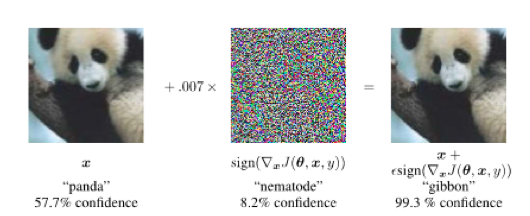
\includegraphics[height=2.5cm]{panda.png}
	\caption{Adversarial example crafting with fast gradient sign \cite{goodfellow2014}.}
	\label{fig:fgsm_craft}
\end{figure}
\subsection{Backpropagated Class Gradient}

The choice of the backpropagated class gradient has direct influence on the generated adversary. In order to reduce the variability of our experiment, we have chosen the true sample label as the backpropagated gradient coupled with the ascent method. The intuition behind this choice is that we look to increase the cost function of the target class by moving away from the current true label. Moreover, in order to test our networks, we needed an $\epsilon$ value that would not only keep the image meaning understandable to human perception but also provide only the minimum amount of perturbation so as to push most of the samples to the closest vicinity leading to a successful misclassification. From all the trials performed, the value of $\epsilon$ that seemed to fulfil our needs was 0.01. 


\section{Results}
The baseline of our comparison is done through the performance of a balanced network to adversarial attacks. Table~\ref{tbl:results} shows that the accuracy for all classes is drastically reduced when the balanced model is presented with adversarial examples. The effectiveness of the adversarial attack can be partially explained by the balancing of the dataset . In a model where the dataset used in training aims for normalization over all classes, the network is often caught in trying to find weights and biases that generalizes well over all set of labels. Therefore, small perturbations become more efficient due to a bigger proximity of classes distributions in space.


\subsection{Class under-sampling and over-sampling}



Networks with under-sampled datasets were more vulnerable when presented with adversarial examples. Figure~\ref{fig:relative_difference} shows the relative difference for all the three networks (balanced, under-sampled and over-sampled). Values were calculated by finding the difference between the perturbed accuracy and the non-perturbed accuracy of each class model. They represent the percentage on which the initial accuracy was reduced. The under-sampled model had the higher relative difference on average, which shows that the imbalanced nature of the dataset ended-up increasing the vulnerability of the model.

Class imbalanced models are naturally affected by the false positive and false negative trade off shown on figure~\ref{fig:class_dist}. The decision boundaries on such models favour the class with more samples and, hence, increases the accuracy for one class while decreasing for the other classes. The area under the curve for misclassified examples on the under-sampled distribution is bigger, and it is caused by the suboptimal exploration of feature space of that class. This effect is exploited by adversaries as there is an increase on the misclassification rate of distributions with lower amplitude. An under-sample of a specific label causes its distribution to be squished into space and, hence, have less impact on the definition of decision boundaries.


\begin{table}
	\centering
	
	\begin{tabular}{lccccc}
		\toprule
		&\multicolumn{2}{c}{Different Model}
		&\multicolumn{3}{c}{Same Model}
		\\\cmidrule(r){2-3}\cmidrule(l){4-6}
		Class Label &Undersample &Oversample &Balanced &Undersample &Oversample \\
		\midrule
		0 - Airplane &60\%& 87\% &36\%& 19\%    & 61\% \\
		1 - Automobile &64\%& 91\% &23\%& 16\%    & 63\% \\
		2 - Bird &38\%& 73\% &20\%& 9.4\%    & 27\% \\
		3 - Cat &21\%& 72\% &11\%& 0.5\%    & 19\% \\
		4 - Deer &58\%& 80\% &20\%& 9.8\%    & 20\% \\
		5 - Dog &47\%& 76\% &15\%& 9\%    & 38\% \\
		6 - Frog &76\%& 88\% &27\%& 20\%    & 49\% \\
		7 - Horse &59\%& 88\% &20\%& 18\%    & 52\% \\
		8 - Ship &69\%& 89\% &37\%& 19\%    & 59\% \\
		9 - Truck &46\%& 87\% &49\%& 21\%    & 54\% \\
		\bottomrule
		\hfill
	\end{tabular}
	\caption{Results for the two different sources of perturbations along with the two different imbalanced datasets}
	\label{tbl:results}
\end{table}
\begin{figure}
	\centering
	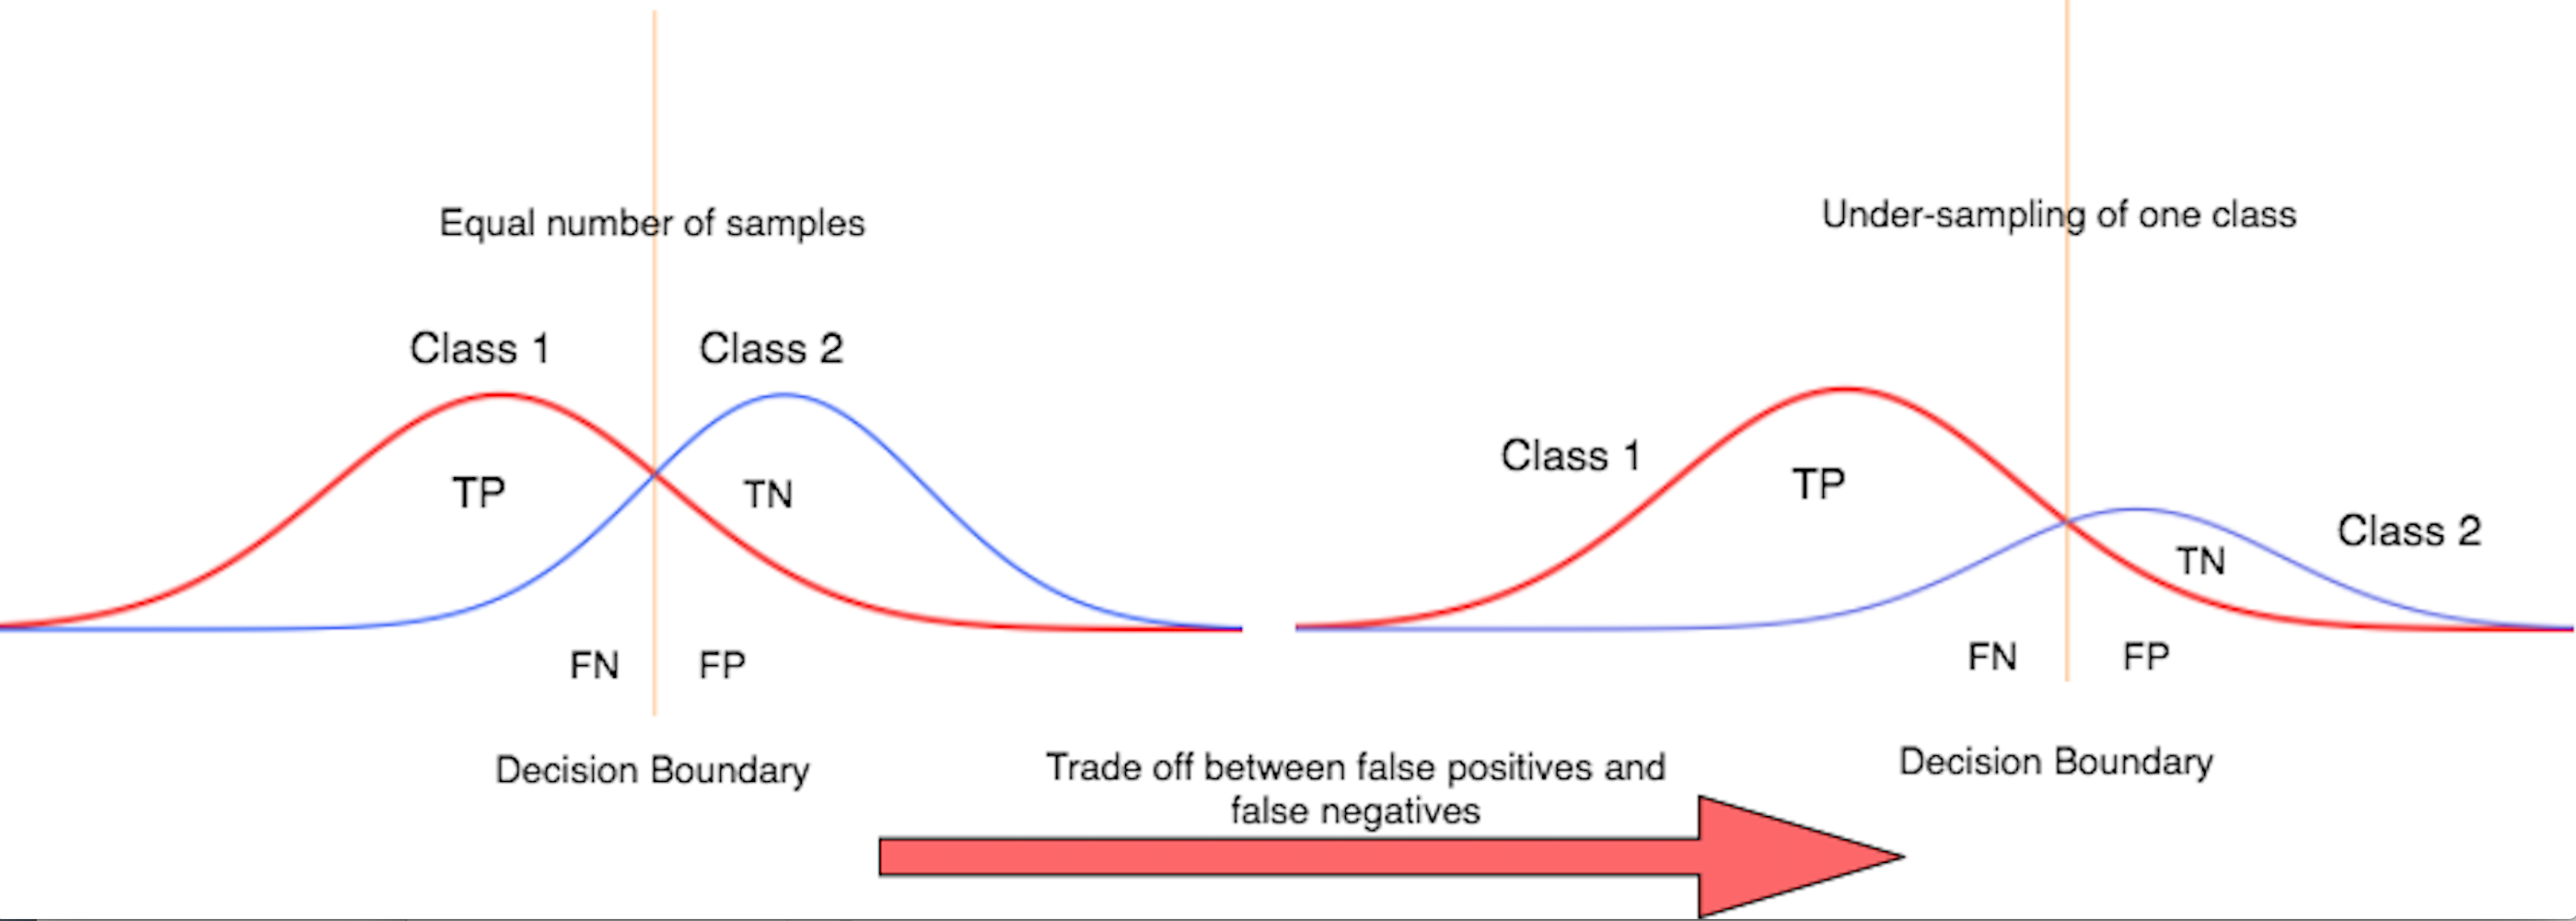
\includegraphics[height=4cm]{class_dist.png}
	\caption{Dataset imbalance causes models to perform adjustments of decision boundaries leading to an increase on accuracy of the majority class and decrease on the minority class.}
	\label{fig:class_dist}
\end{figure}


Perturbation on the over-sampling case had a weaker effect, as the small push caused by our $\epsilon$ was not enough to move points to outside of their distributions. Objects of the over-sampled classes would need bigger steps in order to successfully create an adversarial that leads to a wrong classification label. Accuracy for most of the over-sampling cases was around 45\% and the relative difference was the lowest of all three models, which shows robustness of the target over-sampled class.



\begin{figure}
	\centering
	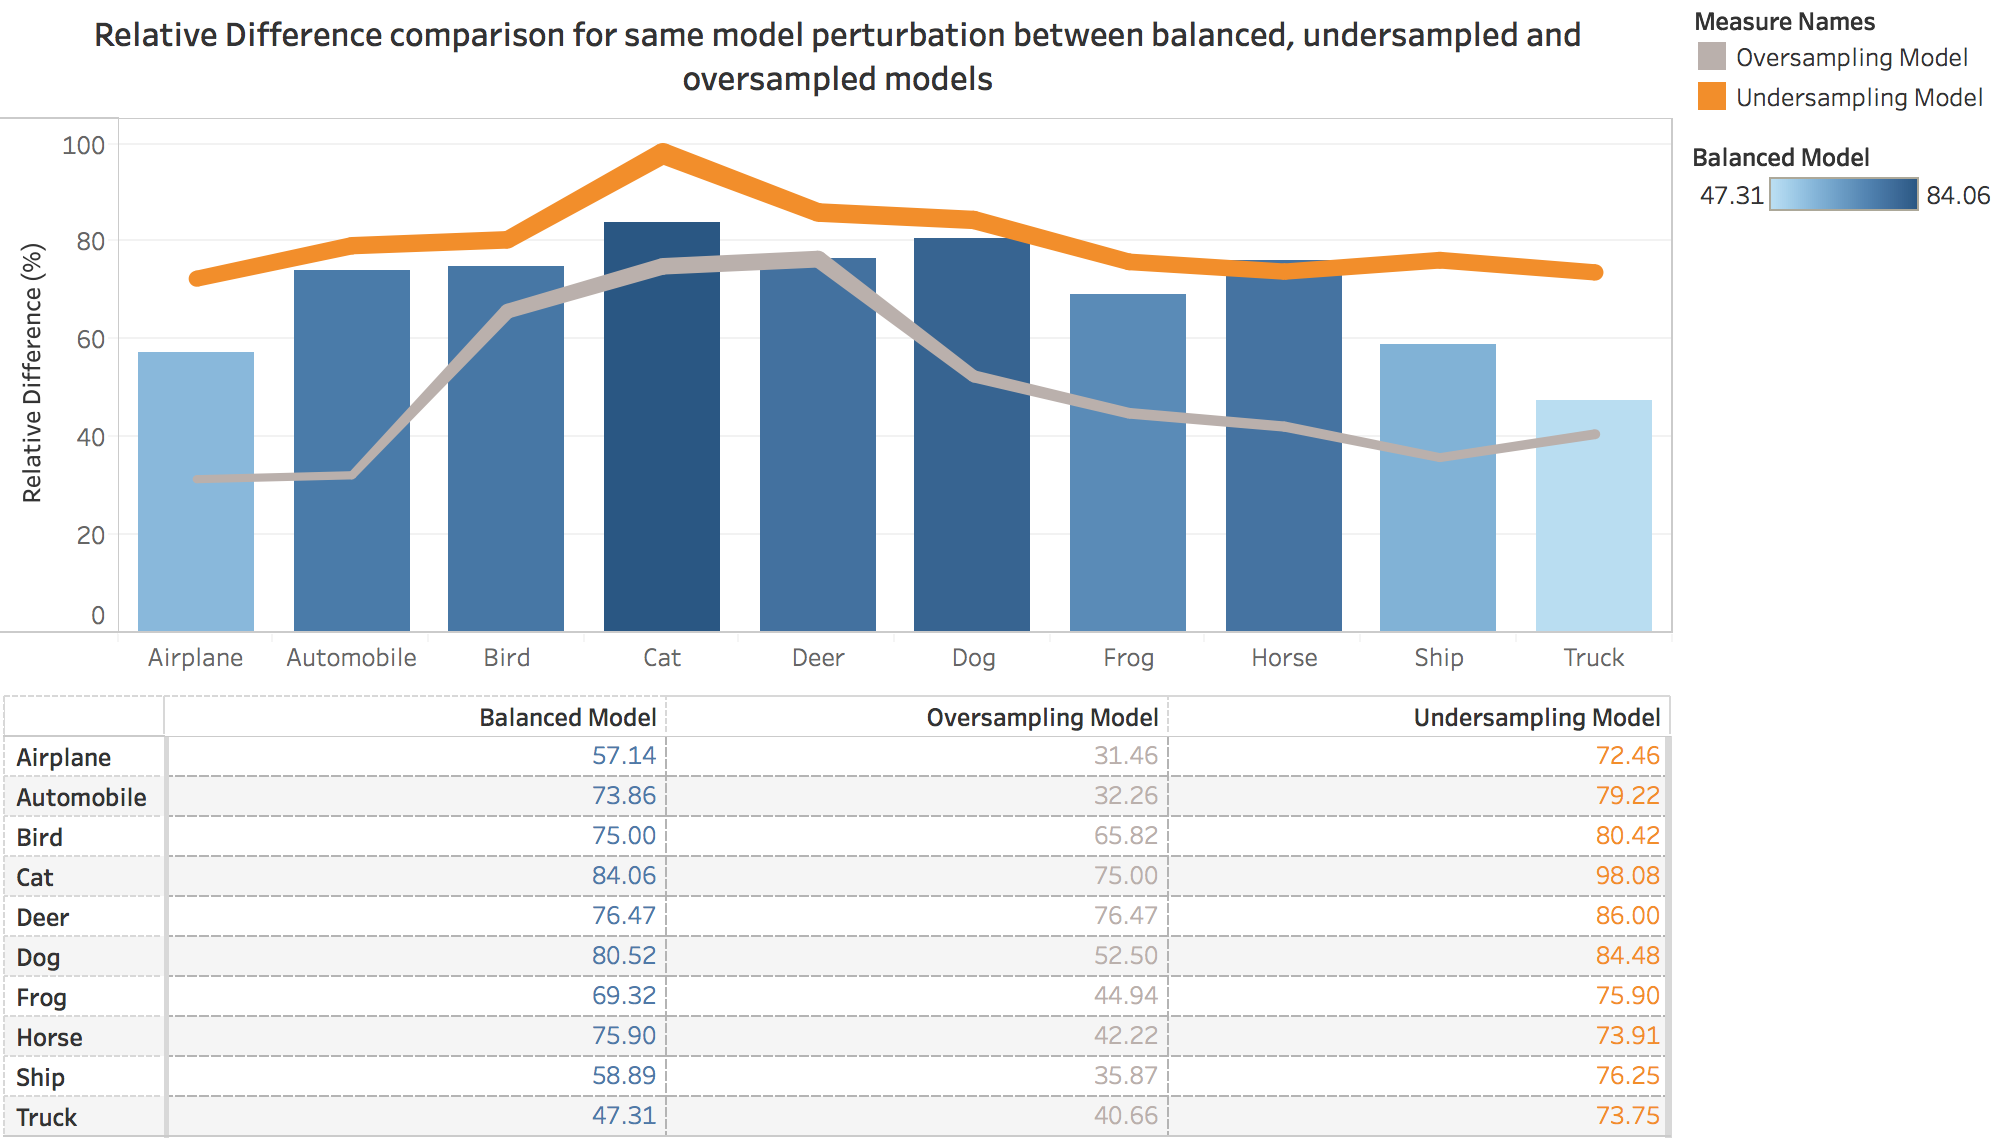
\includegraphics[height=6.5cm]{rel_diff_graph.png}
	\caption{Relative difference for each model. Higher numbers means more vulnerability}
	\label{fig:relative_difference}
\end{figure}


The increased number of samples of the over-sampled label causes the network to perform a trade-off when optimizing its loss function. For instance, the decision boundary would be chosen in order to minimize the total error of the network. The cost function is lower when the decision boundary minimizes the misclassification of the majority class as there is a higher number of samples. The choice of a biased decision boundary could be one of the factors explaining the higher resilience of over-sampled networks.

\subsection{Transfer Learning}

The use of a different model for creating adversaries has shown less effective when compared to the same model attack. As the overall gradient have not only different direction but also magnitudes, the attacked system has proven to be more robust. The experiment reveals that although Gradient Sign is quite effective for fooling networks it does require a good amount of knowledge from the underlying training parameters so as to unleash its full potential. 
\begin{figure}
	\label{fig7} 
	\begin{minipage}[b]{0.5\linewidth}
		\centering
		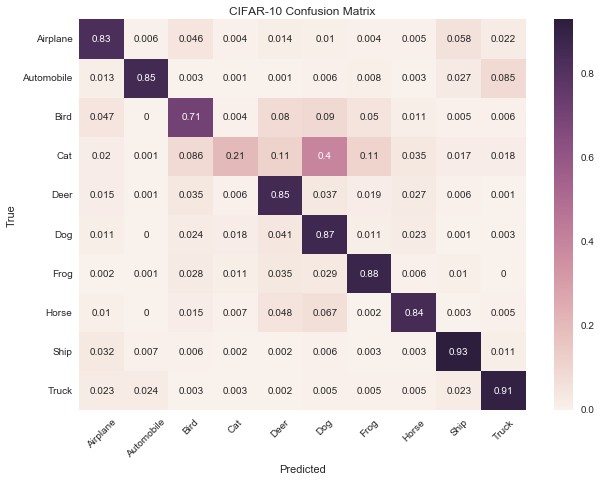
\includegraphics[width=1\linewidth]{cat_undersampling_per.png} 
	\end{minipage}%%
	\begin{minipage}[b]{0.5\linewidth}
		\centering
		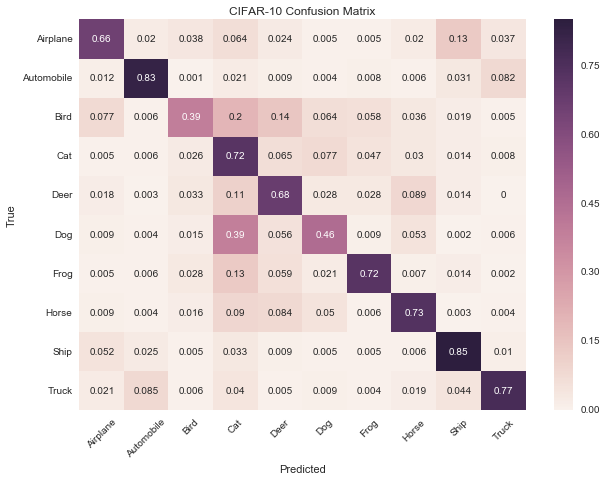
\includegraphics[width=1\linewidth]{cat_oversampling_per.png} 
	\end{minipage} 
	\begin{minipage}[b]{0.5\linewidth}
		\centering
		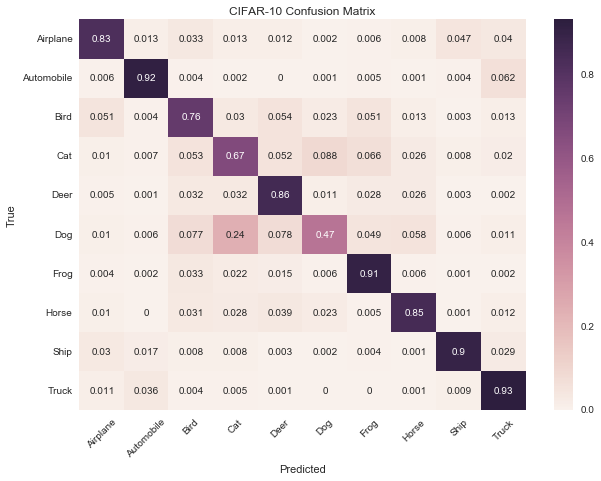
\includegraphics[width=1\linewidth]{dog_undersampling_per.png} 
	\end{minipage}%% 
	\begin{minipage}[b]{0.5\linewidth}
		\centering
		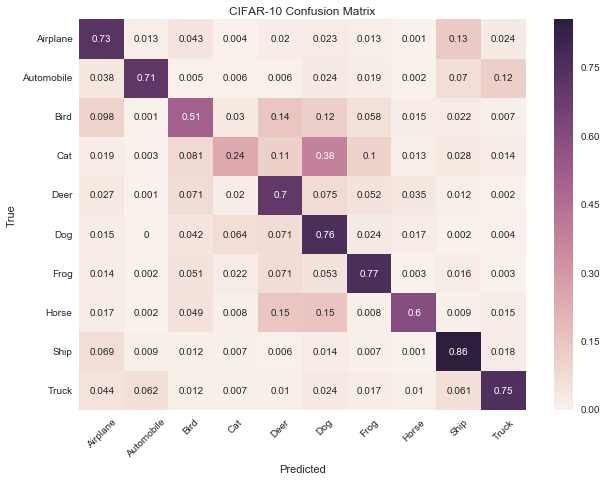
\includegraphics[width=1\linewidth]{dog_oversampling_per.png} 
	\end{minipage} 
	\centering
	\caption{Top left and right: cat under-sampling / over-sampling with perturbation. Bottom left and right: dog under-sampling / over-sampling with perturbation}
	\label{fig:overlap}
\end{figure}
Attacking an under-sampled/over-sampled network with the gradient of the balanced network did not show to be as effective as using the same model's gradient. The average accuracy of an under-sampled model attack with adversaries generated from a different network was 53.8\% while the same metric was 25.8\% for the same model attack. Even that our training samples are within the same data domain, there are still huge differences on the gradients learned from the network. 



\subsection{Overlapping distributions}

When classes in the dataset already have distributions that are very similar to one another the effects of adversaries seems to be even stronger. Figure~\ref{fig:conf_matrix_full} shows that for the pairs cat/dog and automobile/truck, misclassification naturally happens towards one another due to similarities in their feature space. On this case, our experiment shows that the adversarial attacks intensifies this phenomenon by increasing the number of times on which one class is picked over another. Figure~\ref{fig:overlap} shows that both cat and dogs are increasingly misclassified between themselves when under-sampled datasets on both classes are used. While on the cat under-sampling case 40\% of the samples were misclassified as dogs, on the oversampling 39\% of the dogs were misclassified as cats. This results gives interesting insights, as it shows that the gradient sign is navigating around the target class distribution and when an overlap occurs it becomes easier to create an adversarial to the class with higher similarities.


\section{Conclusion}

This work sheds an important light on machine learning methods. Several real-life models are deeply concerned with possible vulnerabilities of their models, and studies on this field were being done for the past 20 years. Still, the imbalance learning problem remains one of the big questions in machine learning. Adversarial attacks are one more concern for those working with such systems, but they could also be seen as a tool that could forcibly make a model to stretch its occupation over the data domain space when we add adversaries to our training set \cite{goodfellow2016}. Every new threat to predictive techniques is also a new improvement over model generalisation capabilities as the creation of the former could be used to improve the latter. Imbalanced datasets can be seen as one way of understanding adversarial attacks, as the lack of knowledge on a specific label seems to increase models vulnerabilities to such attacks

\section{Future Work}
Deep Neural Nets are seen by most people as black-box models as it is really hard to reason about what the model is actually learning. Tools like adversarial methods helps to extract insights from such methods and should be explored further. This work has performed tests on a dataset with a small number of classes, and in the future, datasets like ImageNet could be used to confirm our insights or discover new ones. The excessive amount of parameters in DNNs do not shield them from one of the most common effects in machine learning models - the domain shift caused by unseen data points. We strongly believe that the studies of adversaries could greatly help the understanding of the boundaries of such models.


\bibliographystyle{splncs03} 
\bibliography{refs}

\end{document}
